% -------------------------------------------------------------------------------------
\chapter{Related work} \label{chap:related_work}
% -------------------------------------------------------------------------------------

In this chapter, we will go in-depth discussing common approaches that are being used in the group recommendation task. Firstly, we specify the main approaches and divide them into groups by how they approach the transition from single-user preferences to group results.
Then we mention the main simple techniques and describe how they interact with the usual recommendation approaches. Lastly, we dive into more advanced methods that perform the aggregation more elaborately.

\section{Categories} \label{sec:03_categories}
We assume that we have individual user preferences (if group preferences are available, then the task becomes a simple recommendation with the group acting as a single user); therefore, it is necessary to make a distinction based on where the algorithm goes from the preference of the group's users to a result for the whole group.

We can put each algorithm into one of the following three groups based on the aggregation step:
\begin{itemize}
    \item \textbf{Aggregate models} \newline
    The aggregation works on merging the preferences of each group member into a single set of preferences that a recommender system can directly consume, therefore creating a group preference model. Aggregating the single-user preferences either directly by aggregating ratings of seen, or rated items, or by aggregating the extracted models of user preference to create a single model for the whole group, such as preference matrix in matrix factorization approaches, text descriptions, or item-based recommendations and so on, we will discuss these techniques later.
    
    
    This aggregation step precedes the recommendation step. We can see a visualization in Figure \ref{fig:before_rec_agg}.
    
    
    \item \textbf{Aggregate predictions} \newline
     Aggregates predictions outputted from RS. Recommender recommends separately for each group member based solely on their single-user preferences. Then the resulting recommended items are aggregated into a single list of recommendations for the whole group. There are two main ways how the final list can be created. Either directly take items recommended to each user and append them together in some specified manner, or the second way, calculate some utility function from all recommended items and select those most fitting to the group based on this utility function. We will discuss both in more detail in Section \ref{sec:03_simple_aggregation_metods}.
     
     The aggregation step follows after the actual recommendation step. We can see a visualization of this approach in Figure \ref{fig:after_rec_agg}.
     
    \item \textbf{Aggregation is a uniform part of the recommender} \newline
    In this case, the algorithm directly works with group users and does not allow for a clear distinction of the aggregation step. It is deeply and inseparably built into the algorithm itself. Sometimes the perception of the inseparability of these two steps can vary in the literature. For example, aggregating the user profiles in matrix factorization makes the aggregation inseparable because there is a specific preprocessing done before the aggregation step. However, others will point out that the user latent matrix is just a representation of a user preference, even if processed by the algorithm itself. We will let the reader decide where they see the distinguishing border. We will briefly discuss the available methods in \ref{sec:03_advanced_methods}
\end{itemize}


This presented grouping based on the aggregation step is different from the related literature  \cite{recommendations_to_groups-jameson2007}, and \cite{grouprecommendersystems_felfernig2018group}, where they also make a distinction into three groups but based on the data that the aggregation processes and the position. Instead, we have chosen a little different distinction based more on the interaction of the aggregation with the recommender system, essentially putting two groups from the literature mentioned above under a single group (\textit{aggregate models}), but with the mentioned possible subdivision.
    

\begin{figure}[htbp]
    \centering
    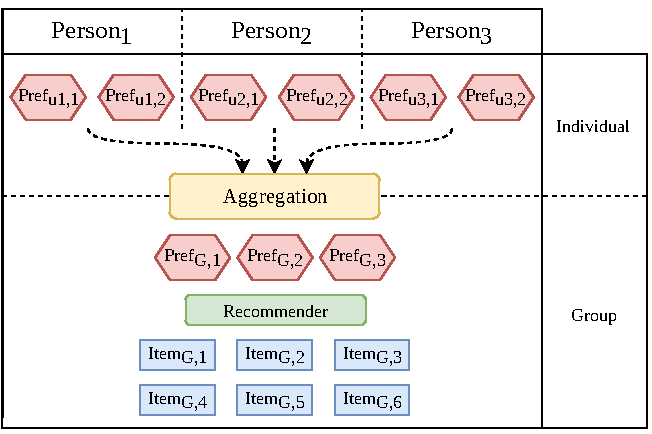
\includegraphics{img/before-rec-aggregation.pdf}
    \caption{High-level overview of group recommendation with aggregation of individuals' preferences, before recommendation.}
    \label{fig:before_rec_agg}
\end{figure}

\begin{figure}[htbp]
    \centering
    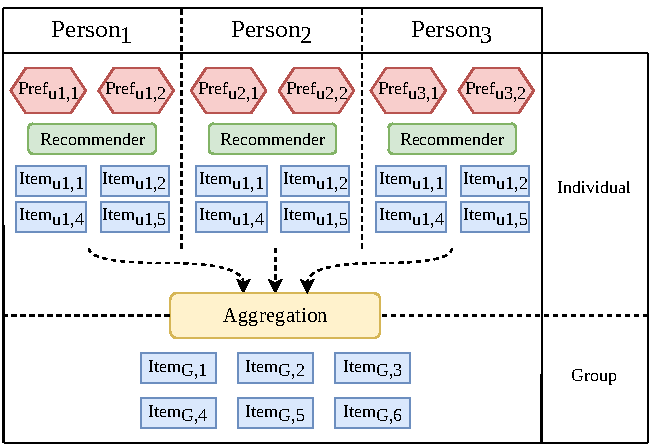
\includegraphics{img/after-rec-aggregation.pdf}
    \caption{High-level overview of group recommendation with aggregation on top of recommendation results for individual users.}
    \label{fig:after_rec_agg}
\end{figure}






\section{Simple aggregation methods}\label{sec:03_simple_aggregation_metods}
We will now introduce the main aggregation functions (interchangeably as 'aggregation strategies', 'aggregation methods') used, together with an overview of how they interact with the single-user recommender systems introduced in Subsection \ref{subsec:01_rec_sys.main_alg_approaches}.

\subsection{Methods}\label{subsec:03_simple_aggregation_methods.methods}

Aggregation methods can be divided into three groups based on their high-level approach: majority-based, consensus-based, and borderline-based strategies. The majority-based generally uses the most popular item among the group members, the consensus-based considers the preferences of all the group members, and the borderline-based considers a subset of the items by some limiting criteria.

We now list the most common aggregation methods as mentioned in \cite{grouprecommendersystems_felfernig2018group}, \cite{masthoff_2011_group_rec_systems} and \cite{masthoff_2004_group_modeling} specify to which of the group mentioned above they belong.
%The common aggregation methods as mentioned in \cite{grouprecommendersystems_felfernig2018group}, \cite{masthoff_2011_group_rec_systems} and \cite{masthoff_2004_group_modeling} are:

\begin{itemize}
    \item \textbf{Additive utilitarian} (ADD, consensus)\newline
        Sum of scores for an item across the group
        \begin{equation}
            \argmax_{i \in I}{\sum_{u \in G}{\textrm{score}(u,i)}}
        \end{equation}
    
    \item \textbf{Approval Voting} (APP, majority)\newline
        Number of users that like the item above a certain threshold
        \begin{equation}
            \argmax_{i \in I}{
                \big\lvert{\left\{
                    u \in G : \textrm{score}(u,i) \geq \textrm{treshold}
                \right\}}\big\rvert
            }
        \end{equation}
    
    \item \textbf{Average} (AVG, consensus)\newline
        Average of scores for an item across the group
        \begin{equation}
            \argmax_{i \in I}{\dfrac{\sum_{u \in G}{\textrm{score}(u,i)}}{\abs{G}}}
        \end{equation}
    
    \item \textbf{Average without Misery} (AVM, consensus)\newline
        Average of scores for an item across the group only if the item is above a certain threshold for all group members
        \begin{equation}
            \argmax_{ i \in I : \nexists u \in G | \textrm{score}(u,i) \leq \textrm{treshold}}{
                \dfrac{\sum_{u \in G}{\textrm{score}(u,i)}}{\abs{G}}
            }
        \end{equation}
        
    \item \textbf{Borda count} (BRC, majority)\newline
        Sum of scores derived from item rankings. The ranking score is defined for each user by ordering the user's items by score and awarding points corresponding to the item's location in this ordered list. The worst item receives 1 point, and the best item $|I|$ points.
        \begin{equation}
                \argmax_{i \in I}{\left(\sum_{u \in G}{\textrm{RankingScore}(u,i)}\right)}
            \end{equation}
        Where \textit{ranking score} is defined as follows:
        \begin{equation*}
            \textrm{RankingScore}(u,i) := 
            \big\lvert{\left\{
                i_{other} \in I : \textrm{score}(u,i_{other}) \leq \textrm{score}(u,i)
            \right\}}\big\rvert
        \end{equation*}
    
    \item \textbf{Copeland rule} (COP, majority)\newline
        Difference between the number of wins and losses for pair-wise comparison of all items
        \begin{equation}
            \argmax_{i \in I}{
                \big(\textrm{W}(t, I - t) - \textrm{L}(t, I - t)\big)
            }
        \end{equation}
    
    \item \textbf{Fairness} (FAI, consensus)\newline
        Users, in turn, one after another, select their top item.
        \begin{equation}
            \argmax_{i \in I}{{\textrm{score}(u_{current},i)}}
        \end{equation}
        Where $u_{current}$ is the user selected from $G$ for each iteration according to some (in most cases circular or ping pong) rule.
    
    \item \textbf{Least misery} (LMS, borderline)\newline
        Uses the lowest received rating among the group members as the item's aggregated rating.
        \begin{equation}
            \argmax_{i \in I}{\left(\min_{u \in G}{\left(\textrm{score}(u,i)\right)}\right)}
        \end{equation}
    
    \item \textbf{Most Pleasure} (MPL, borderline)\newline
        It uses the highest received rating among the group members as the item rating.
        \begin{equation}
            \argmax_{i \in I}{\left(\max_{u \in G}{\left(\textrm{score}(u,i)\right)}\right)}
        \end{equation}
        
    \item \textbf{Majority Voting} (MAJ, majority)\newline
        Uses the rating given by the majority of the group's members. (Can only work on discrete ratings)
        \begin{equation}
            \argmax_{i \in I}{\left(\mode_{u \in G}{\left(\textrm{score}(u,i)\right)}\right)}
        \end{equation}
    
    \item \textbf{Most Respected Person} (MRP, borderline)\newline
        Uses rating proposed by the most respected member of the group.
        \begin{equation}
            \argmax_{i \in I}{\textrm{score}(u_{most\_respected},i)}
        \end{equation}
        
        
    \item \textbf{Multiplicative} (MUL, consensus)\newline
        Multiplies all received ratings together.
        \begin{equation}
            \argmax_{i \in I}{\left(\prod_{u \in G}{\textrm{score}(u,i)}\right)}
        \end{equation}
        
        
    \item \textbf{Plurality Voting} (PLU, majority)\newline
        Each user has a set number of votes that get distributed. The item with the most received votes is selected.
        \begin{equation}
            \argmax_{i \in I}{\left(\sum_{u \in G}{\textrm{VotesAwarded}(u,i)}\right)}
        \end{equation}
        
        Where \textit{votes awarded} is some function that decides for each user how the available votes will be distributed among the items.
        
\end{itemize}

Some of the methods have an additional distinguishing factor: they are iterative calculations instead of a single calculation that returns the final ordering. Most notably \textit{Fairness}, it calculates the next item purely from a currently selected user, users changing in iterations one after another. Another one is \textit{Plurality Voting}, this technique can also be iterative, but it is not mandatory. After the top item is selected, we reset the calculation, therefore iteratively selecting top items. All the other ones are single-iteration methods, where the final list requires only one calculation.

Now we will show how these strategies work together with an RS to provide a complete group recommender system, which will serve as an introduction to the inner workings of such a system in order for us to continue towards more advanced aggregation methods.

\subsection{Usage with recommender systems}
We now need to distinguish between \textit{model aggregation} and \textit{prediction aggregation} due to, in most cases, very different inputs and required outputs from the aggregation.
\subsubsection{Prediction aggregation}
In most cases, we use them as \textit{prediction aggregation} after the recommendation is relatively straightforward. In all (to us known) cases, RS returns recommended items together with some sort of rating of the recommendation. There are some applications where this presumption does not hold, such as building a group recommendation aggregation on top of a \textit{black box} recommender that only returns a list of items, for example, if extracting recommended items data from a web page where we only retrieve the list itself and we do not have access to the underlying recommender system. Nevertheless, in the following section, we will assume that we have full access to the rating data of the outputted items. We further assume that, if necessary, we can acquire ratings and an ordering for all possible items.

As shown in Figure \ref{fig:after_rec_agg}, we first get a list of recommended items (together with ratings) for each user. Then we can directly apply the methods mentioned in Subsection \ref{subsec:03_simple_aggregation_methods.methods}.

\subsubsection{Model aggregation}
Running aggregation on top of user preferences, instead of lists of recommended items, is more challenging due to the many possible inputs the recommender can take, such as explicit or implicit feedback. As discussed in Section \ref{sec:03_categories}, we have two main options, aggregation of ratings and aggregation of mined preferences.

The first option is the aggregation of ratings, in other words creating a set of ratings representing the whole group. This approach is preferred due to its simplicity. We can use many of the previously mentioned simple methods, mainly the \textit{consensus-based}, which aggregate ratings directly (positive and negative). Other mentioned methods can be used as well. However, some of them do not make much sense to adapt, for example, the voting-based, with which we will be very limited due to the usual sparsity of the feedback ratings that we have available.

The second option, the aggregation of mined preferences, is more present in content-based systems. We aggregate not the rating but some other data that represent the users' likes and dislikes. As an example, we will use the \textit{tf-idf} keyword extraction which is by far the most popular method used in the text-based recommendation as mentioned in \cite{beel_2016_rs_literature_survey}. We can weight \textit{tf-idf} concepts extracted from the user feedback by the received rating and then aggregate these concepts together for the whole group. As we can see, it is a more elaborate approach that requires more modifications to the simple methods mentioned.



\section{Advanced methods}\label{sec:03_advanced_methods}
As we can see, the simple methods mentioned before are pretty straightforward. They have mostly straightforward and clear objectives and try to optimize in different ways, some quite vaguely specified goals. However, as discussed in Chapter \ref{chap:fairness}, the objective is quite hard to define and measure. We will now introduce other methods that either directly or indirectly try to optimize some better-specified goal.

\subsection{GFAR} \label{subsec:03_advanced_methods.gfar}
So far, we have introduced methods that do not directly specify any form of optimization in the direction of \textit{fairness}. A new method introduced in\cite{GFAR-kaya2020} directly optimizes the resulting list to balance the relevance of the recommended items in a rank-sensitive way. Similarly to all before mentioned methods, it is an aggregation approach that works on top of a single user RS.

\subsubsection{Introduction}

As mentioned, the authors focus on the \textit{fairness} of $\mathit{topN}_G$ (\textit{fairness} of the top N recommended items for group G). Where they define \textit{fairness} as a property of the top-$N_G$ items, not just any single item but the whole list. As already discussed in Section \ref{sec:01_rec_sys}, the difference between optimization independently item after item versus in some way for the whole list can yield significantly better results when used in sequential consumption of items or balancing users with different preferences.

In the latter case of a member with differing preferences, we have more freedom to compensate and give more priority for balancing fairness towards this one user if we define fairness as a property of the whole list.

This kind of fairness is the main focus of the GFAR algorithm. In a way, it exceeds this by trying to optimize each prefix of the recommendation list. We will later define categories based on this fairness perception in Chapter \ref{chap:our_work}. The GFAR algorithm is to us, the only known algorithm that optimizes this kind of prefix fairness we call \textit{rank-sensitive} fairness.

In Subsection \ref{subsec:03_simple_aggregation_methods.methods}, we have already mentioned the FAI algorithm that tries to balance the fairness of the whole list. It generates the aggregated results in steps, each following step maximizing the utility of the following user in turn. This approach solves the problem mentioned above very simply by not considering the group preferences at all. It is just trying to please everyone in turns, not considering if the rest of the group will like the item in that turn. 


\subsubsection{Approach}

What if we have instead considered the previously recommended items when selecting the next one in the list? The authors propose defining \textit{fairness} together with ordering within the group by saying that "a $\mathit{topN}$ is fair to a group if the relevance of the items is balanced across the group members for \textit{each prefix} of the $\mathit{topN}_G$. In other words, for each iteration, we try to select an item that improves the balance as much as possible.

Let us first define Borda relevance following \cite{xiao_2017_fairness_aware_g_rec} as:

\begin{equation}
    \textrm{Borda-rel}(u,i) &= \big\lvert{
            \left\{j : \textrm{rank}(j, \textrm{topN}_u) < \textrm{rank}(i, \textrm{topN}_u) \right\}, \forall_j \in \textrm{topN}_u)
        }\big\rvert
\end{equation}

Where $\mathit{topN}_u$ is a list of top N items for user $u$, rank is the position of item $i$ in the user's $u$ candidate list (position is determined by ordering the items based on the returned items score, from the best to the worst, where the best receives a rank of 1). Borda relevance essentially gives zero points to the last item and increases the points by one for each position up in the list, with the first/top item getting $(N - 1$) points. We can calculate Borda-rel from rank simply by $\textrm{Borda-rel}(u,i) = N - rank(u,i)$. Note that if there are items that have the same rank, then the maximum value has to be awarded to the group in order to translate this way to Borda-rel.

Now we can set the probability of item $i$ being relevant for user $u$ as:

\begin{equation}
    p(\textrm{rel}|u, i) = \frac{\textrm{Borda-rel}(u, i)}{\sum_{j \in \textrm{topN}_u}{\textrm{Borda-rel}(u, j)}}
\end{equation}

Let also $p(\neg\textrm{rel}|u, S)$ be the probability that item $i$ is not relevant for any of the items in set $S$. We derive the probability that at least one item from set $S$ is relevant to the user $u$ as:

\begin{equation} \label{eq:atleast_one_relevant}
\begin{aligned}
    p(\textrm{rel}|u, S) &= 1 - p(\neg\textrm{rel}|u, S) \\
    & = 1 - \prod_{i \in S}{(1 - p(\textrm{rel}|u, i))}
\end{aligned}
\end{equation}

Now we want to generalize for the whole group, so we define $f(S)$ as the sum of probabilities for each user that they find at least one relevant item in the set $S$:

\begin{equation} \label{eq:relevance_for_set}
\begin{aligned}
    f(S) &= \sum_{u \in G}{\left(1 - p(\neg\textrm{rel}|u, S)\right)} \\
    & = \sum_{u \in G}{\left(1 - \prod_{i \in S}{(1 - p(\textrm{rel}|u, i))}\right)}
\end{aligned}
\end{equation}

We have used Group G as a constant in Equation \ref{eq:relevance_for_set}, and forward, the group will stay the same during the calculation. $f(S)$ shows how to balance the fairness amongst the group members for a specified set of items. We now want to extend it in order to make it rank-sensitive by defining a marginal gain in function $f$ for adding a new item $i$ to the set $S$ as follows:

\begin{equation} \label{eq:relevance_for_set_add}
\begin{aligned}
    f(i, S) &= f(S \cup {i}) - f(S) \\
    & = \sum_{u \in G}{\left[p(\textrm{rel}|u, i) \prod_{j \in S}{(1 - p(\textrm{rel}|u, j))}\right]}
\end{aligned}
\end{equation}

Where we have used Equations \ref{eq:atleast_one_relevant} and \ref{eq:relevance_for_set}, finally, we can define an ordered set that is considered fair if it balances each of its prefixes. In other words, the first item of the set should be considered fair/balanced by all group members as much as possible, then the first two items, and so on. We define fairness in an ordered set $OS$ as:

\begin{equation}
    \textrm{fair}(OS) = \sum_{k=1}^{|OS|}{f(OS)[k], \{i \in OS : \textrm{rank}(i, OS) < k\})}
\end{equation}


% \subsection{Package-to-Group Recommendations}
% Paper \cite{serbos_2017_fairness_packages_to_group_rec}?


\subsection{XPO} \label{subsec:03_advanced_methods.xpo}
% Paper \cite{sacharidis_2019_top_n_with_fairness}?
The last algorithm performed a greedy search based on the probability of at least one item being relevant for each user in order to find balance among users in a rank-sensitive way.

The following method introduced in \cite{sacharidis_2019_top_n_with_fairness} XPO and its variant NPO are aggregation approaches that explore a simple but intuitive notion of fairness that utilizes Pareto optimality of item's raking in all admissible ways in which a group may reach a decision.

\subsubsection{Introduction}
The authors specifically aim to minimize the feeling of dissatisfaction, which somehow differs from the majority of previous works that aim to optimize the group's overall satisfaction or, more recently, from works that aim to optimize fairness for each group member.

With a measure utility for each pair of users and item, we have a group utility to be the average member utility according to \cite{social_welfare} and fairness to be the minimum member utility, which is equal to the Least misery approach.

With these definitions, the measure of utility itself becomes important as it is the main factor that we are optimizing on. If we have a recommender system that recommends top-K items for each user, then for a set of recommended items N, the utility of that user is the similarity between the top-K list and list N.

There are multiple similarity measures for comparing two lists, such as symmetrical measures, Spearman's foot rule, rho, and Kendall's tau. Furthermore, unsymmetrical, better-known precision, recall, and normalized discounted cumulative gain.

The authors' approach is based on the notion of Pareto optimality. Pareto optimal item for the group is an item that ranks the highest according to all group members. The group unanimously agrees that no other item would be sharply better than this one.

Therefore this Pareto optimality is inherently fair due to all members considering the item the best. However, most usually, items are always a different set of trade-offs that need to be balanced.

Let us now be more specific and present the algorithms' details.

\subsubsection{Approach}

The authors assume that the system is providing us with a top-N list of recommendations for each member $m$ of a group $\mathcal{G}$. This set of items is considered \textit{ground truth}. Each item is considered a vector in m-dimensional space $\R^n$, where each dimension is a rank $r_u(i)$ of the item in the user's top-N list of items. If an item is not in that list, then rank of N+1 is awarded. For completeness, rank is a position in the ordered list of top-N items of each user, therefore the best item has a rank 1, second best has a rank of 2 and the last item has a rank N. We assume this rank for each user independently only based on theirs top-N items.

For a group we get candidate items as
\begin{equation} \label{eq:top-N_candidates}
    \mathcal{C}_\mathcal{G} = \bigcup_{u\in \mathcal{G}} \mathit{topN}(u).
\end{equation}


Further, we say that an item $i$ dominates item $i'$ according to a group $G$ if
\begin{equation}
\forall u \in \mathcal{G}: r_u(i) \leq r_u(i') 	\land \exists u' \in \mathcal{G}: r_{u'}(i) < r_{u'}(i') 
\end{equation}
It means that ranks for all users must be equal or better, but for at least one user, the rank needs to be sharply better.

A good question might arise, why the equality even matters if items are ranked based on their position in a sorted list? Two situations can arise. Either the utility is exactly the same, and therefore the items will be in the same position, or the items are not in the top-N for that user. In the latter case, we award the rank of N+1 as already mentioned, and there can, and most probably will be, many items sharing this lowest rank.

Further, when evaluating an aggregation strategy, we say that it is Pareto-efficient if whenever an item $i$ is ranked higher than another item $i'$ by each group member, then also the strategy rates the item $i$ higher than item $i'$. Pareto optimal strategy respects the Pareto domination of items described before.

This property Pareto-efficiency is respected by all rating and rank aggregation strategies. We can easily see that if a strategy recommends an item that is Pareto dominated by another one (is better, by rank and or rating), then it has recommended a subpar item and therefore is not optimal, based on the underlying rating.

We call a set of items that are not dominated by any other items Pareto optimal (PO). One interesting side note that the authors do not address: does always at least one Pareto optimal item exist? We see that PO property is transitive, therefore if an item $i$ dominates a set of some items $I$, then if there is an item $i'$ that dominates $i$, then from the transitivity, it also dominates all items from the set $I$. And so on, therefore there always exists an item or a set of items that are Pareto optimal. In a different way, we can view this relationship as an acyclic-directed graph.

Next, they define \textit{N-level Pareto optimal} (N-lPO) set, which contains items that are dominated by at most $N - 1$ other items. Note that N-lPO set contains items from all smaller PO sets, such as \textit{3-lPO} $\subset$ \textit{2-lPO} $\subset$ \textit{1-lPO}.

We can calculate the N-lPO level for each item by comparing it with all other items from the set and directly calculating the number of times other items dominated the current one. This, unfortunately, leads to $\mathcal{O}(n^2)$ time complexity, where n is the size of the candidate set. It would be interesting to investigate the possibility of using the transitivity property cleverly to get better time complexity, at least in the average case, but that is outside of the scope of this work.

Ideally, we would want to take the N-lPO from all the items, but that would require to first have a ranking of all items for each user, and then calculating the Pareto optimally level between all pairs of items, which would be very computationally expensive. We, therefore, take an approximation of the N-lPO set of items from the candidate set where for each user we request their top-N where N is larger than the final required recommendation size or as large as computationally feasible.

The next step is the interesting part of the authors' new method, they consider all \textit{linear aggregation strategies}, where linear strategy assigns weight $w_u$ to each user so that the total weight sums to 1, then item raking is multiplied user-wise with this weight and summed up as

\begin{equation}
    1 = \sum_{u \in \mathcal{G}} w_u.
\end{equation}

Then items score under this linear strategy $\mathcal{L}_w$ is
\begin{equation}
    S_\mathcal{L}(i) = \sum_{u \in \mathcal{G}} w_u r_u(i).
\end{equation}

Each linear aggregation strategy can be uniquely represented by the weight $w$.

The motivation behind considering all linear aggregation strategies is to get the ratio for items that do not dominate each other. When two items lie on the same Pareto level, it does not mean they achieve the same average score over all l. strategies. We can use this ratio to further distinguish between the items and therefore compare items even when they are on the same Pareto level. We can see an illustration for 6 items and two users in Figure \ref{fig:xpo_example}. Item $i_1$ and $i_2$ lie on the Pareto front and therefore there is not clear which item is better. But for only one linear strategy in this case, with weight $w$ the items will have the same score. For any other weight vector, there will be a clear winner. We, therefore, want to compute this ratio. We can compute this two-dimensional case analytically as $3/7$ and $4/7$ for weight $w = (3/7, 4/7)$. We can see that only Pareto optimal items would have a non-zero probability, and for every non-Pareto optimal set of items, there would be a clear winner.

\begin{figure}[htbp]
    \centering
    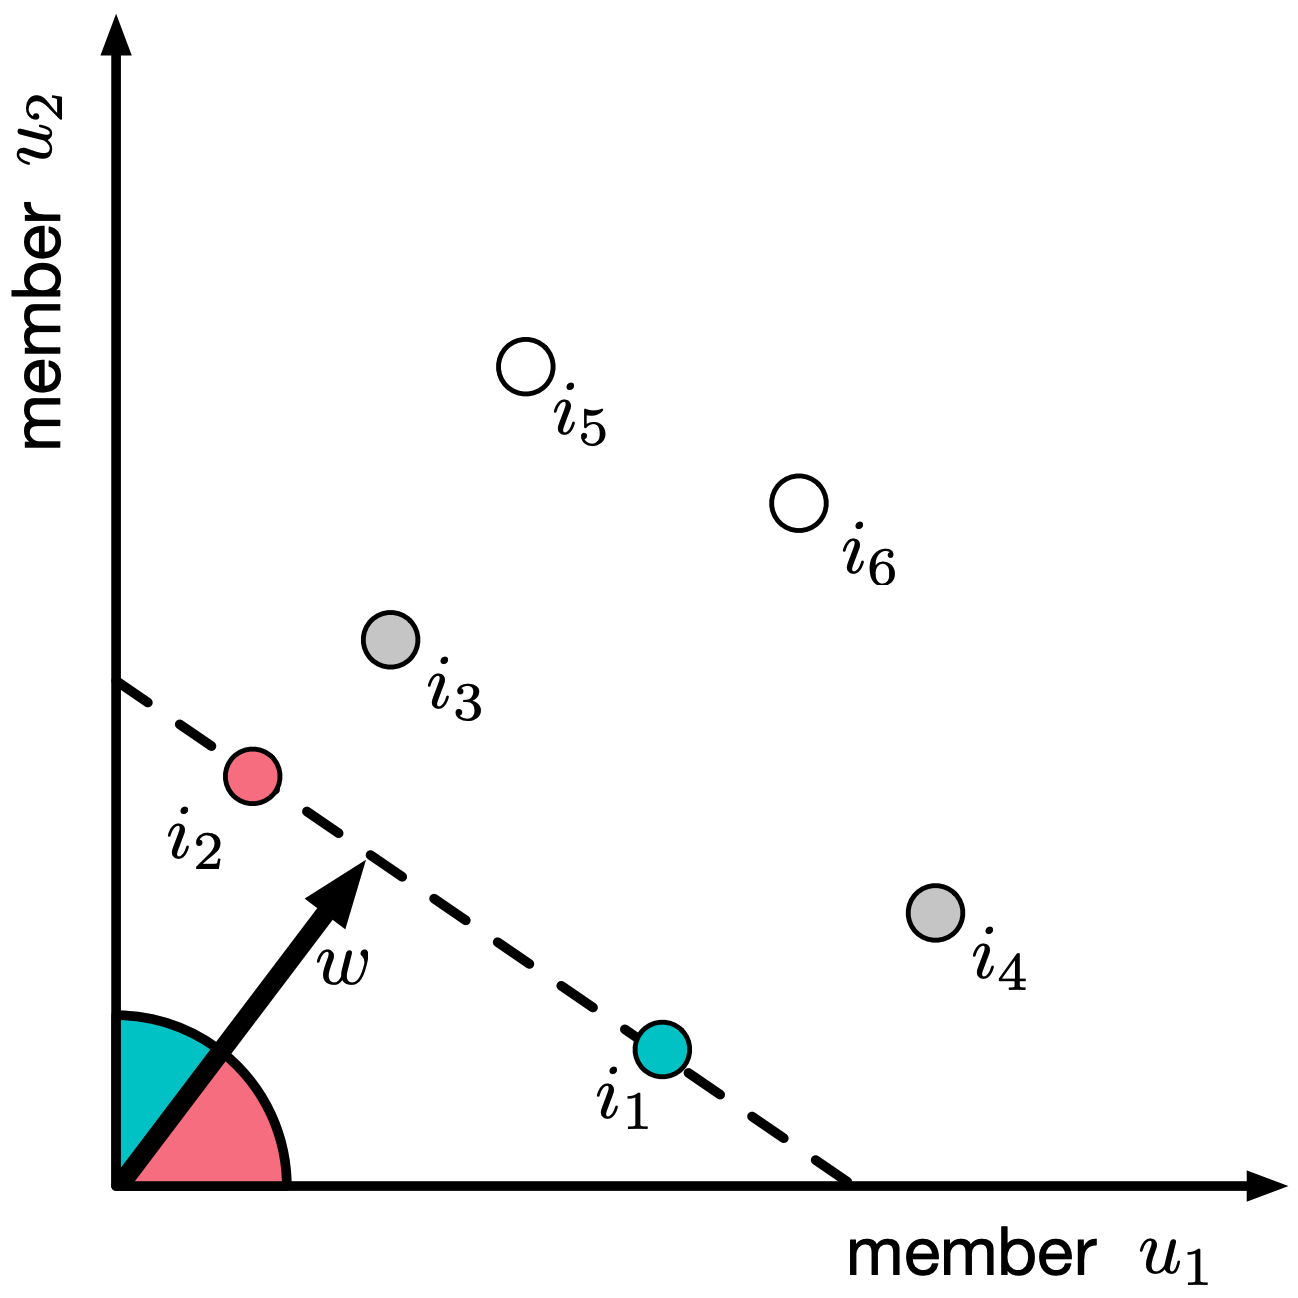
\includegraphics[width=2.5in]{img/XPO_las.png}
    \caption[Example of 6 items based on two group members $u_1$ and $u_2$ from \cite{sacharidis_2019_top_n_with_fairness}.]{Example of 6 items based on two group members $u_1$ and $u_2$ from \cite{sacharidis_2019_top_n_with_fairness}. Item $i_2$ is Pareto optimal for user $u_1$, and item $i_1$ is Pareto optimal for $u_2$.}
    \label{fig:xpo_example}
\end{figure}


In 2 dimensional case, computing the exact probability is possible, but in a multidimensional case, the problem does not have a simple analytical solution. Therefore considering all possible weights is unpractical in order to get an average of items rating across all linear strategies, we opt for a Monte Carlo method of computing this probability.

Therefore, we generate many random weights, each representing a different linear aggregation strategy. For each $\mathcal{L}_w$ we compute how many times an item $i$ ended up being in the \textit{top-N} where  $N$, in this case, is the desired size of the recommended list.

Items are then rated by how many times each N-PO item ranks within the \textit{top-N}. Best N items are returned as the output of the group recommender strategy. We call this approach N-level Pareto optimal aggregation (NPO).

The size of N-level Pareto optimal items can be much larger than the required size of output N, we therefore can perform a binary search to identify the smallest $x \in [1, N]$ for which there are at least the desired amount of items N. We can formulate this as 

\begin{equation} \label{eq:xpo}
    argmin_{x=1}^{N} |\mathcal{P}_x| \geq N,
\end{equation}
where $\mathcal{P}_x$ represents the set of \textit{x-level Pareto optimal} items. We call this aggregation strategy XPO.

Note, the only difference between NPO and XPO is the smaller candidate final candidate selection step. The initial candidate list drawn from top-N candidates for each user $\mathcal{C}_\mathcal{G}$ stays identical.


\subsection{D'Hondt direct optimization (FuzzDA)} \label{subsec:03_advanced_methods.DHondtDO}

This method directly uses a definition of fairness that is widely around the world as a mandate allocation strategy for elections and the division of a discrete number of mandates/items.

It focuses on D'Hondt's algorithm (DA) which is commonly used in European elections. DA is a greedy selection algorithm that minimizes the number of votes that need to be left aside so that the remaining votes are represented exactly proportionally as described in \cite{wiki:dhondt_method}.

The procedure behind DA works as follows: in steps, it awards the party with the largest quotient $quot$ one seat, and after each step, the quotient is recalculated. The quotient is calculated as follows:

\begin{equation}
    quot(V_p, s_p) = \dfrac{V_p}{s_p + 1},
\end{equation}
where $V_p$ is the total number of votes that party $p$ received and $s_v$ is the number of seats that have been allocated to party $p$ so far (initially 0).

In order to compensate for this, FuzzDA presented in \cite{fuzz_da}, can be used. For each group member $u$ and each candidate item $i$, we assign a relevance score of that item for that user to $r_{u,i} \in [0,1]$. At each step, FuzzDA select a candidate that maximizes $\sum_{u \in G} quot(V_u, s_u) * r_{u,i}$. After each step, each group members' accountable votes are decreased by the factor of $r_{u,i}$. This represents a fuzzy approach that fixes the DA problem of being unable to handle items that are relevant to multiple parties by lowering their accountable votes (therefore the power in the next step) by how much utility they have received with each new item.
